\section{Skuteczność metod obrony}
W kolejnym etapie badano skuteczność metod obrony, których celem było zminimalizowanie poziomu \gls{ASR} otrzymanego dla ataków na wybrane modele bez dodatkowej ochrony. Pierwszym badanym podejściem była technika Self-Reminder. Otrzymane wyniki przedstawiono w tabeli~\ref{tab:self_reminder_comparison_tab}.
\begin{table}[!ht]
    \centering
    \begin{tabular}{l|c|c|c|c}
        \hline
        \multirow{2}{*}{Model + metoda obrony}   & \multicolumn{4}{c}{ASR [\%]}                    \\\cline{2-5}
                                                 & Podstawowo                   & DAN & GCG & PAIR \\\hline
        Llama-3.1-8B-Instruct + Self-Reminder    & 3                            & 43  & 1   & 32   \\\hline
        Mistral-7B-Instruct-v0.3 + Self-Reminder & 7                            & 76  & 17  & 61   \\\hline
    \end{tabular}
    \caption{\label{tab:self_reminder_comparison_tab}Skuteczność badanych metod ataku z zastosowaniem metody obrony Self-Reminder}
\end{table}
Zauważyć można, że po zastosowaniu tej ochrony, poziom \gls{ASR} spadł dla każdego z badanych ataków. Szczególnie wyróżnić można spadek tego wskaźnika z poziomu 49\% do zaledwie 7\% w przypadku modelu Mistral-7B-Instruct-v0.3 dla bezpośrednich szkodliwych poleceń. Wyraźnie zredukowano również skuteczność ataku \gls{GCG} dla obu modeli, dla Llama-3.1-8B-Instruct udało się zablokować ten atak niemal w całości. Natomiast pomimo zastosowania tego podejścia do obrony, oba modele wykazują sporą podatność na ataki \gls{DAN} oraz \gls{PAIR}. W przypadku Mistral, metoda \gls{PAIR} omija zabezpieczenia w 61\% przypadków, a \gls{DAN} w aż 76\%. Skuteczność tych ataków w przypadku modelu Llama wyniosła natomiast odpowiednio 43\% oraz 32\%. Wywnioskować można, że technika Self-Reminder pozwala zadowalająco obronić \gls{LLM} przed bezpośrednimi niebezpiecznymi zapytaniami, natomiast nie jest wystarczającą ochroną przed iteracyjnymi metodami omijania zabezpieczeń oraz podejściami opartymi na inżynierii promptów. Do zapobiegania takim atakom wymagane są bardziej skuteczne metody obrony.

Sprawdzono w następnym kroku skuteczność obrony przy użyciu zewnętrznego modelu moderacyjnego Llama-Guard-3-8B. Rezultaty zaprezentowano w tabeli~\ref{tab:guard_comparison_tab}.
\begin{table}[!ht]
    \centering
    \begin{tabular}{l|c|c|c|c}
        \hline
        \multirow{2}{*}{Model + metoda obrony} & \multicolumn{4}{c}{ASR [\%]}                    \\\cline{2-5}
                                               & Podstawowo                   & DAN & GCG & PAIR \\\hline
        Llama-3.1-8B-Instruct + Llama-Guard    & 1                            & 0   & 0   & 21   \\\hline
        Mistral-7B-Instruct-v0.3 + Llama-Guard & 1                            & 1   & 1   & 33   \\\hline
    \end{tabular}
    \caption{\label{tab:guard_comparison_tab}Skuteczność badanych metod ataku na modele chronione przez Llama Guard}
\end{table}
Zastosowanie zewnętrznego modelu zapewniło wysoki poziom bezpieczeństwa. Dla bezpośrednich poleceń, \gls{DAN} oraz \gls{GCG} udało się zredukować poziom skuteczności ataków do blisko 0\%. W przypadku tego rozwiązania, osięgnięto zbliżony poziom ochrony przed tymi atakami dla obu modeli. Niezależnie od tego czy modelem docelowym był Llama czy Mistral, sukces ominięcia zabezpieczeń spadł do poziomu od 0 do 1\%. Zauważyć natomiast można, że atak \gls{PAIR} nadal jest wysoce skuteczny i potrafi ominąć zabezpieczenia modelu docelowego oraz moderacyjnego. Technika \gls{PAIR} dla modelu Llama-3.1-8B-Instruct bronionym przez Llama-Guard-3-8B osiągnęła poziom \gls{ASR} wynoszący 21\%, natomiast w analogicznym scenariuszu dla modelu Mistral-7B-Instruct-v0.3 otrzymano \gls{ASR} równe 33\%. Pokazuje to, że automatyczne i iteracyjne dostosowywanie poleceń wejściowych może skutecznie omijać modele pomimo chronienia ich przez dedykowane modele moderacyjne.

Finalnie zbadano skuteczność ataków na modele z zastosowanym mechanizmem obronnym opartym na inżynierii aktywacji. Wyniki zestawiono w tabeli~\ref{tab:act_comparison_tab}.
\begin{table}[!ht]
    \centering
    \begin{tabular}{l|c|c|c|c}
        \hline
        \multirow{2}{*}{Model + metoda obrony}            & \multicolumn{4}{c}{ASR [\%]}                    \\\cline{2-5}
                                                          & Podstawowo                   & DAN & GCG & PAIR \\\hline
        Llama-3.1-8B-Instruct + sterowanie aktywacjami    & 3                            & 1   & 14  & 28   \\\hline
        Mistral-7B-Instruct-v0.3 + sterowanie aktywacjami & 42                           & 95  & 70  & 78   \\\hline
    \end{tabular}
    \caption{\label{tab:act_comparison_tab}Skuteczność badanych metod ataku na modele chronione mechanizmem opartym na inżynierii aktywacji}
\end{table}
W przypadku modelu Llama osiągnięto ochronę na wysokim poziomie. Największą różnicę w skuteczności ataku można dostrzec dla \gls{DAN}, gdzie po dodaniu sterowania aktywacjami zanotowano spadek \gls{ASR} aż o 54 punkty procentowe redukując tą podatność prawie w całości. Przy użyciu bezpośrednich szkodliwych instrukcji ominięto zabezpieczenia w dwóch przypadkach więcej niż podczas ataku \gls{DAN}. W każdym z tych 3 poleceń bramka sterująca wskazała, że intencja zapytania nie jest szkodliwa i nie aktywowała metody obrony. Skuteczny okazał się znowu automatyczny atak \gls{PAIR}, który przełamał obronę w 28\% przypadków. Jest to spadek o 7 punktów procentowych w stosunku do scenariusza, w którym nie zastosowano metody obrony.
Sterowanie aktywacjami nie ochroniło wystarczająco skutecznie natomiast modelu Mistral. Jest to zapewne spowodowane słabszym treningiem \gls{LLM} pod kątem bezpieczeństwa. Pokazuje to, że skuteczność sterowania aktywacjami jako metoda obrony jest zależna od podstawowego dostrojenia modelu. Dowodzi to, że jest to technika, która wzmocnić może podstawowe, wbudowane bezpieczeństwo modelu, lecz nie jest jego zamiennikiem. Zauważyć to można na podstawie rezultatów dla modelu Llama, który początkowo miał już wysoki poziom bezpieczeństwa, a dodatkowe sterowanie aktywacjami pozytywnie wpłynęło na spadek powodzenia ataków. Największą różnicę między tymi modelami można dostrzec w przypadku wyników ataku \gls{DAN}. Mistral uległ w aż 95\% przypadków, a bramka sterująca oznaczyła intencję jako szkodliwą w jedynie 11 z nich. Natomiast dla modelu Llama bramka poprawnie sklasyfikowała intencję dla 99\% ataków \gls{DAN}, czego skutkiem była tylko jedna niebezpieczna odpowiedź. Brak silnych mechanizmów odmowy wpłynął negatywnie na finalną skuteczność metody obrony modelu Mistral przy pomocy sterowania aktywacjami.

Otrzymane rezultaty \gls{ASR} dla badanych metod ataków i obrony zostały zestawione w tabeli~\ref{tab:all_comparison_tab} oraz na wykresie~\ref{fig:asr_defense}.
\begin{table}[!ht]
    \centering
    \begin{tabular}{l|l|c|c|c|c}
        \hline
        \multirow{2}{*}{Model} & \multirow{2}{*}{Metoda obrony} & \multicolumn{4}{c}{ASR ($\Delta$ASR) [\%]}                                                                                                                                                                                           \\\cline{3-6}
                               &                                & Podstawowo                                             & DAN                                                     & GCG                                                     & PAIR                                                    \\\hline
        \multirow{3}{*}{Llama-3.1-8B-Instruct}
                               & Self-Reminder                  & 3 \textcolor{ForestGreen}{\scriptsize($\downarrow$3)}  & 43 \textcolor{ForestGreen}{\scriptsize($\downarrow$12)} & 1 \textcolor{ForestGreen}{\scriptsize($\downarrow$12)}  & 32 \textcolor{ForestGreen}{\scriptsize($\downarrow$3)}  \\\cline{2-6}
                               & Llama-Guard                    & 1 \textcolor{ForestGreen}{\scriptsize($\downarrow$5)}  & 0 \textcolor{ForestGreen}{\scriptsize($\downarrow$55)}  & 0 \textcolor{ForestGreen}{\scriptsize($\downarrow$13)}  & 21 \textcolor{ForestGreen}{\scriptsize($\downarrow$14)} \\\cline{2-6}
                               & Sterowanie aktywacjami         & 3 \textcolor{ForestGreen}{\scriptsize($\downarrow$3)}  & 1 \textcolor{ForestGreen}{\scriptsize($\downarrow$54)}  & 14 \textcolor{Red}{\scriptsize($\uparrow$1)}            & 28 \textcolor{ForestGreen}{\scriptsize($\downarrow$7)}  \\\hline
        \multirow{3}{*}{Mistral-7B-Instruct-v0.3}
                               & Self-Reminder                  & 7 \textcolor{ForestGreen}{\scriptsize($\downarrow$42)} & 76 \textcolor{ForestGreen}{\scriptsize($\downarrow$20)} & 17 \textcolor{ForestGreen}{\scriptsize($\downarrow$58)} & 61 \textcolor{ForestGreen}{\scriptsize($\downarrow$24)} \\\cline{2-6}
                               & Llama-Guard                    & 1 \textcolor{ForestGreen}{\scriptsize($\downarrow$48)} & 1 \textcolor{ForestGreen}{\scriptsize($\downarrow$95)}  & 1 \textcolor{ForestGreen}{\scriptsize($\downarrow$74)}  & 33 \textcolor{ForestGreen}{\scriptsize($\downarrow$52)} \\\cline{2-6}
                               & Sterowanie aktywacjami         & 42 \textcolor{ForestGreen}{\scriptsize($\downarrow$7)} & 95 \textcolor{ForestGreen}{\scriptsize($\downarrow$1)}  & 70 \textcolor{ForestGreen}{\scriptsize($\downarrow$5)}  & 78 \textcolor{ForestGreen}{\scriptsize($\downarrow$7)}  \\\hline
    \end{tabular}
    \caption{Skuteczność badanych metod ataku wobec wdrożonych metod obrony wraz ze spadkami ($\downarrow$) lub wzrostami ($\uparrow$) punktów procentowych względem poziomu bazowego.}
    \label{tab:all_comparison_tab}
\end{table}
\begin{figure}[!ht]
    \centering
    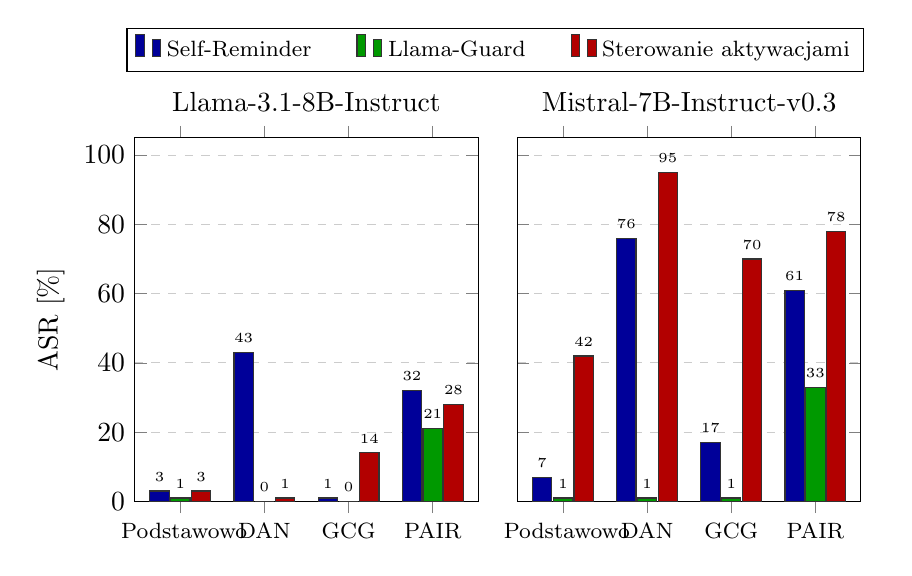
\begin{tikzpicture}
        \pgfplotsset{
            asr plot/.style={
                    ybar=0.5pt,
                    bar width=7pt,
                    width=0.49\textwidth,
                    height=6.2cm,
                    ymin=0,
                    ymax=105,
                    symbolic x coords={Podstawowo, DAN, GCG, PAIR},
                    xtick=data,
                    x tick label style={font=\footnotesize, text width=1.5cm, align=center},
                    ytick={0, 20, 40, 60, 80, 100},
                    ymajorgrids=true,
                    grid style={dashed, gray!40},
                    nodes near coords,
                    every node near coord/.append style={font=\tiny, /pgf/number format/fixed},
                    enlarge x limits=0.18,
                }
        }

        \begin{axis}[
                asr plot,
                name=plot1,
                title={Llama-3.1-8B-Instruct},
                ylabel={ASR [\%]},
                legend style={
                        at={(1.05, 1.18)},
                        anchor=south,
                        legend columns=3,
                        /tikz/every even column/.append style={column sep=0.5cm},
                        font=\footnotesize
                    },
            ]
            % Self-Reminder
            \addplot[fill=blue!60!black, draw=black!80] coordinates {
                    (Podstawowo, 3) (DAN, 43) (GCG, 1) (PAIR, 32)
                };
            % Llama-Guard
            \addplot[fill=green!60!black, draw=black!80] coordinates {
                    (Podstawowo, 1) (DAN, 0) (GCG, 0) (PAIR, 21)
                };
            % Sterowanie aktywacjami
            \addplot[fill=red!70!black, draw=black!80] coordinates {
                    (Podstawowo, 3) (DAN, 1) (GCG, 14) (PAIR, 28)
                };
            \legend{Self-Reminder, Llama-Guard, Sterowanie aktywacjami}
        \end{axis}

        % 2. Wykres po prawej: Mistral-7B-Instruct-v0.3
        \begin{axis}[
                asr plot,
                at={(plot1.south east)},
                xshift=0.5cm,
                title={Mistral-7B-Instruct-v0.3},
                yticklabels={},
            ]
            % Self-Reminder
            \addplot[fill=blue!60!black, draw=black!80] coordinates {
                    (Podstawowo, 7) (DAN, 76) (GCG, 17) (PAIR, 61)
                };
            % Llama-Guard
            \addplot[fill=green!60!black, draw=black!80] coordinates {
                    (Podstawowo, 1) (DAN, 1) (GCG, 1) (PAIR, 33)
                };
            % Sterowanie aktywacjami
            \addplot[fill=red!70!black, draw=black!80] coordinates {
                    (Podstawowo, 42) (DAN, 95) (GCG, 70) (PAIR, 78)
                };
        \end{axis}
    \end{tikzpicture}
    \caption{Porównanie wskaźnika ASR dla badanych metod obrony i ataku dla modeli Llama-3.1-8B-Instruct oraz Mistral-7B-Instruct-v0.3.}
    \label{fig:asr_defense}
\end{figure}
Najlepszą metodą pod względem redukcji skuteczności ataków dla każdej z metod ataku okazał się zewnętrzny model moderacyjny Llama-Guard. Zniwelował on dla obu modeli praktycznie wszystkie próby ominięcia zabezpieczeń przez bezpośrednie szkodliwe instrukcje, \gls{DAN} oraz \gls{GCG}. Przy użyciu Llama-Guard osiągnięto również najwyższy spadek \gls{ASR}. W modelu Mistral udało się o 95 punktów procentowych zredukować powodzenie ataku \gls{DAN}. Ponadto, przy jego użyciu odnotowano najwyższe spadki \gls{ASR} względem poziomu bazowego w porównaniu do pozostałych metod obrony.  Llama-Guard uległ natomiast atakowi \gls{PAIR}, dla którego otrzymano \gls{ASR} równe 21\% dla modelu Llama oraz 33\% dla Mistral. Jednakże jest to wciąż najniższy poziom dla tego ataku ze wszystkich trzech badanych metod. Dla Self-Reminder i sterowania aktywacjami otrzymano powodzenie ataku większe o odpowiednio 11 oraz 7 punktów procentowych w przypadku modeli Llama. Natomiast dla modelu Mistral wielkość otrzymanego \gls{ASR} dla tych metod obrony była mniejsza o odpowiednio 28 i 45 punktów procentowych. Zastosowanie Llama-Guard pozwoliło osiągnąć w obu modelach zbliżony poziom bezpieczeństwa.
W przypadku modelu Llama-3.1-8B-Instruct podobny poziom ochrony przed atakami osiągnięto przy pomocy mechanizmu opartego na sterowaniu aktywacjami. Różnice w wyniku \gls{ASR} są nieduże, gdyż największa wyniosła 13 punktów procentowych i została odnotowana dla ataku \gls{GCG}, dla którego wykazano brak poprawy. Sterowanie aktywacjami prawie w całości zlikwidowało podatność na atak \gls{DAN}, gdyż tylko 1 przypadek zakończył się udanym atakiem. Dla metody \gls{PAIR} odnotowano w tym scenariuszu umiarkowaną redukcję \gls{ASR} o 7 punktów procentowych. Można wywnioskować, że dla modelu z wbudowanymi mechanizmami bezpieczeństwa, metoda sterowania aktywacjami może być równie dobrą ochroną co model zewnętrzny. Natomiast dla modelu ze słabszym bezpieczeństwem bazowym, takiego jak Mistral, technika sterowania aktywacjami jedynie w małym stopniu zmniejszyła skuteczność badanych ataków. Są to spadki w zakresie od 1 do 7 punktów procentowych w porównaniu do modelu bez wdrożenia tej metody. Jej rezultaty są dostrzegalnie gorsze w porównaniu do pozostałych dwóch metod.
Technika Self-Reminder w przypadku modelu z rodziny Llama odnotowała znaczące zmniejszenie skuteczności ataku \gls{GCG}, ponieważ dla zapewniła spadek o 12 punktów procentowych względem poziomu bazowego, redukując tym samym skuteczność tego ataku do prawie zera. Dla metody \gls{DAN} obniżyła \gls{ASR} również o 12 punktów procentowych, natomiast zmniejszono skuteczność tylko do 43\%.  Zablokowała również dodatkowe 3 bezpośrednie szkodliwe polecenia. Nie uchroniła natomiast modelu przed atakiem \gls{PAIR}, zmniejszając jego powodzenie o jedyne 3 punkty procentowe. Istotny wpływ na bezpieczeństwo modelu w stosunku do poziomu bazowego można zaobserwować w przypadku modelu Mistral. Dla bezpośrednich poleceń zanotowano spadek \gls{ASR} aż o 42 punkty procentowe. Wyraźne polepszenie obrony dostrzec można także analizując rezultat ataku \gls{GCG}, który przełamał obronę 17 razy w porównaniu z 58 w przypadku poziomu bazowego. Istotnie zmniejszono również \gls{ASR} dla metod \gls{DAN} oraz \gls{PAIR}, natomiast model Mistral wciąż nie był na nie odporny, gdyż pierwszy z nich ominął mechanizm obronny aż 76 razy, a drugi z nich 61. Można zauważyć, że metoda Self-Reminder nie jest wystarczającym zabezpieczeniem modelu przed atakami opartymi na dostosowywaniu szkodliwego promptu wejściowego.
Na podstawie rezultatów przedstawionych w tabeli~\ref{tab:all_comparison_tab} można stwierdzić, że atak \gls{PAIR} jest najbardziej odporny na wprowadzane mechanizmy obronne. Niezależnie od wdrożenej metody obrony jego skuteczność jest dla modelu Llama na poziomie od 21 do 32\%, natomiast dla modelu Mistral od 33\% do 78\%.